\section{Theorie}
\label{sec:Theorie}

Es ist bekannt, dass bewegte elektrische Ladungen magnetische Felder erzeugen (z.B. ein bewegtes Elektron).
Dabei lässt sich das Magnetfeld als eine Vektorgröße beschreiben, dessen Richtung und Betrag durch die magnetische Feldstärke $\vec{H}$ beschrieben wird.
Die magnetische Flussdichte wird beschrieben durch

\begin{equation} \label{eq:Flussdichte}
    \vec{B} = \mu \vec{H} = \mu_{0} \mu_{r} \vec{H}
\end{equation}

wobei $\mu$ die \textit{Permeabitlität}, $\mu_{0}$ die \textit{Vakuum-Permeabitlität} und $\mu_{r}$ die \textit{relative Permeabitlität} ist.
Für bewegte Ladungen in einem stromdurchflossenen Leiter gilt das \textit{Biot-Savartsche Gesetz:}

\begin{equation} \label{eq:Biot-Savart-Gesetz}
    \vec{B}(\vec{r}) = \frac{\mu_{0}I}{4pi} \int \frac{d\vec{s} \times \vec{r}}{r^3}
\end{equation}


\begin{minipage}{0.7\textwidth}
    Dabei beschreibt $I$ den Strom, der durch gegebenen Leiter fließt und $d\vec{s}$ das Leiterstück.
\end{minipage}
\begin{minipage}{0.3\textwidth}
    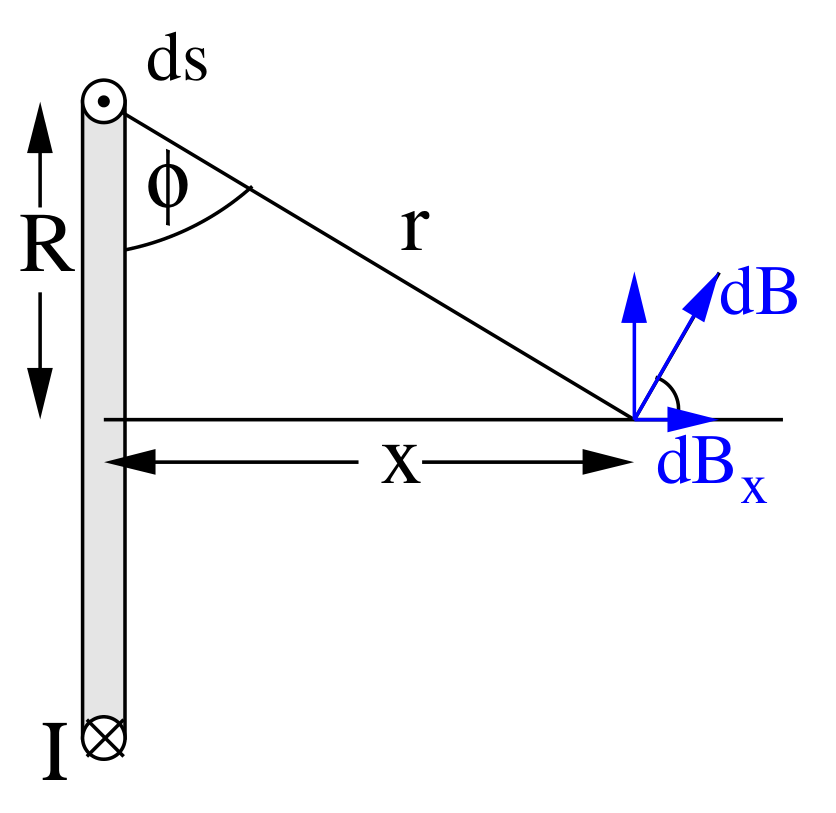
\includegraphics[width=\textwidth]{pictures/BiotSavart1.png}
    \small{Abbildung 1 , Quelle: \cite{sample}}
\end{minipage}

\subsection{Anwendungen vom Biot-Savartschen Gesetz}

Durch die Gleichung (\ref{eq:Biot-Savart-Gesetz}) ergibt sich die wichtige Formel für Leiterschleifen.

\begin{equation} \label{eq:Leiterschleife}
    \vec{B}(x) = \frac{\mu_{0}I}{2} \frac{R^2}{(R^2 + x^2)^{3/2}} \frac{\vec{x}}{|x|}
\end{equation}

Nun ist das Magnetfeld innerhalb stromdurchflossener Spulen annähernd homogen und die Gleichung (\ref{eq:Leiterschleife}) bedarf einer Anpassung.
Außerdem haben wir nun $N$ Windungen und die Spule eine Länge $l$:

\begin{equation} \label{eq:LangeSpule}
    B = \mu_{0}\mu_{r}I \frac{N}{l}
\end{equation}

Dabei ist zu beachten, dass diese Gleichung ihre Gültigkeit außerhalb der Spule verliert, da das Magnetfeld dort inhomogen wird.

Das Magnetfeld der \textbf{Ringspule} lässt sich ebenfalls über das Bio-Savart Gesetz (\ref{eq:Biot-Savart-Gesetz}) berechnen.
Die Ringspule ist charakterisiert durch die Windungszahl $N$ und den Radius $R$.
Man kommt schließlich auf folgende Gleichung:

\begin{equation}
    B = \mu_{0}\mu_{r}I \frac{N}{2\pi R}
\end{equation}

Das Magnetfeld eines \textbf{Helmholtzspulenpaares}, zwei identische Spulen im Abstand $x$ zum Mittelpunkt, berechnet sich wie folgt:

\begin{equation} \label{eq:Helmholtzgleichung}
    B(0) =  B_{1}(x) +  B_{1}(-x) = \frac {\mu_{0} I R^2} {(R^2 + x^2)^{3/2}}
\end{equation}

Dabei ist das Magnetfeld im Idealfall auf der Symmetrieachse nahezu homogen.

\subsection{Ferromagnetische Stoffe}
\textit{Ferromagnetische Stoffe} (wie z.B. Eisen) unterscheiden sich von gewöhnlichen Stoffen.
Zunächst haben sie eine extrem große relative Permeabitlität $\mu_{r}$ und die Gleichung (\ref{eq:Flussdichte}) verliert ihre Gültigkeit.
Solche Ferromagnetischen Stoffe besitzen ein permanentes magnetisches Moment.
Die sogenannten \textit{Weiß'schen Bezirke} richten sich in einzelnen Bereichen parallel zueinander aus.




\begin{minipage}{0.7\textwidth}
    Durch ein äußeres Magnetfeld lässt sich diese Ausrichtung verändern.
    Diese Richtungsänderung geschieht so lange, bis alle Weißschen Bezirke ausgerichtet sind.
    Diese Magnetisierungskurve lässt sich durch eine Hysteresekurve beschreiben.
    Dieser ist rechts schematisch aufgetragen.
    Magnetisiert man ein zuvor unmagnetisiertes Material, wird dieses sich zuerst an der Neukurve (grün) zum Sättigungswert $B_{s}$ bewegen.
    Wird der Strom dann heruntergeregelt, wird sich eine Restmagnetisierung einstellen.
\end{minipage}
\begin{minipage}{0.3\textwidth}
    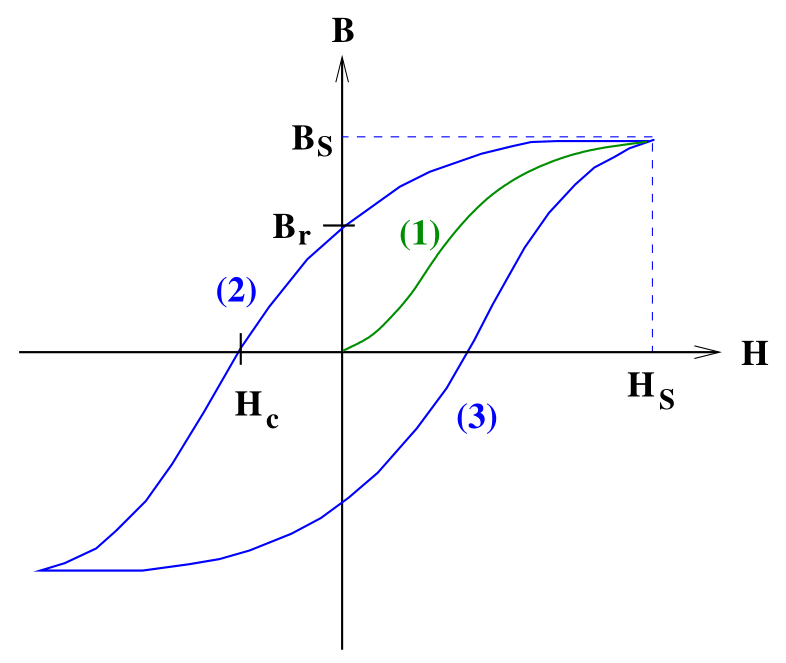
\includegraphics[width=\textwidth]{pictures/Hysteresekurve.png}
    \small{Abbildung 2 , Quelle: \cite{sample}}
\end{minipage}

Diese Restmagnetisierung $B_{r}$ nennt man die Remanenz.
Diese lässt sich durch die \textit{Koerzitivkraft} $H_{c}$ ausgleichen.